\section{UYGULAMA}

Bu bölümde, Coraza WAF log analizi ve SOM kümeleme sisteminin implementasyonu, sistem bileşenlerinin entegrasyonu ve gerçekleştirilen testler detaylı olarak açıklanmaktadır.

\subsection{Sistem Geliştirme Süreci}

Proje, Agile metodoloji kullanılarak aşamalı olarak geliştirilmiştir. Geliştirme süreci üç ana aşamadan oluşmaktadır:

\begin{enumerate}
    \item \textbf{Altyapı Kurulumu:} Jenkins, Coraza WAF ve OWASP ZAP entegrasyonu
    \item \textbf{Analiz Modülü Geliştirme:} Python tabanlı SOM analiz sistemi
    \item \textbf{Web Arayüzü Geliştirme:} Streamlit ile kullanıcı arayüzü
\end{enumerate}

\subsection{Jenkins CI/CD Boru Hattı Uygulaması}

Sistem, iki ana Jenkins boru hattı kullanmaktadır. Ana boru hattı (CorazaWAF-Log-Last) aşağıdaki temel aşamaları içermektedir:

\subsubsection{Ortam Hazırlama ve Bağımlılık Yönetimi}

Boru hattı öncelikle gerekli bağımlılıkları kurar: Python3, \texttt{pip}, Flask ve \texttt{wget} paketleri \texttt{apt} paket yöneticisi ile sisteme yüklenir.

\textbf{Go Sürüm Yönetimi:}
\begin{lstlisting}[language=bash]
LATEST_GO=$(curl -s https://go.dev/VERSION?m=text)
wget https://golang.org/dl/${LATEST_GO}.linux-amd64.tar.gz
sudo tar -C /usr/local -xzf ${LATEST_GO}.linux-amd64.tar.gz
export PATH=$PATH:/usr/local/go/bin
\end{lstlisting}

\subsubsection{Dinamik Servis Oluşturma}

Boru hattı, \texttt{writeFile} direktifi ile dinamik Flask uygulaması oluşturur ve Go tabanlı WAF'ı arka planda çalıştırır. Her iki servis de paralel olarak 8091 ve 8080 portlarında hizmet verir.

\newpage

\begin{figure}[!ht]
    \centering
    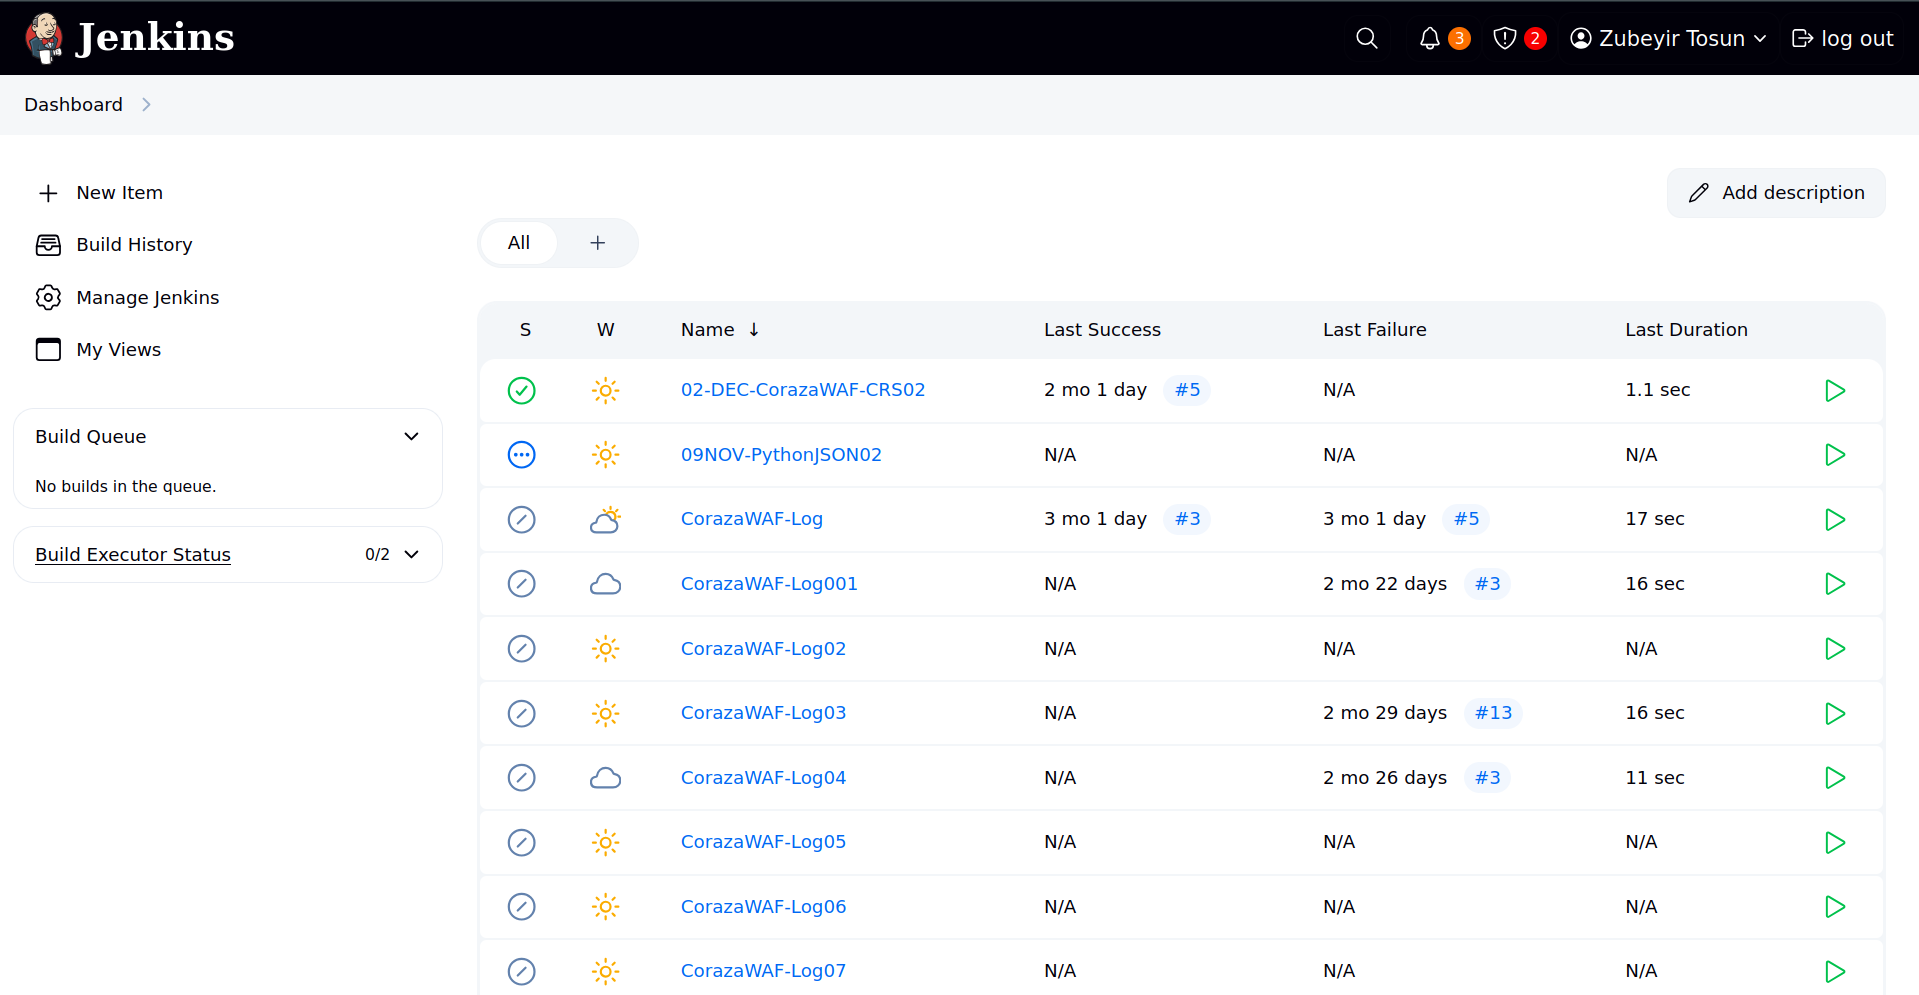
\includegraphics[width=0.8\textwidth]{images/jenkins-dashboard.png}
    \caption{Jenkins Pipeline Dashboard Görünümü}
    \label{fig:jenkins_dashboard}
\end{figure}

Boru hattı çalıştırıldığında, Şekil \ref{fig:jenkins_dashboard}'de görüldüğü gibi Jenkins gösterge paneli üzerinden tüm aşamaların durumu izlenebilmektedir. Gösterge paneli, her boru hattının başarı durumunu, çalışma süresini ve log çıktılarını gerçek zamanlı olarak göstermektedir.

\subsubsection{Çoklu Boru Hattı Yönetimi}

Sistem, dört farklı boru hattı ile tam otomatik dağıtım sağlar:

\begin{itemize}
    \item \textbf{CorazaWAF-Log-Last:} Ana WAF log toplama ve analiz boru hattı
    \item \textbf{Flask-API-Server:} RESTful API servisi
    \item \textbf{ZAP-Security-Scanner:} Otomatik güvenlik tarama modülü
    \item \textbf{Streamlit-Analytics:} Web tabanlı analiz arayüzü
\end{itemize}

Her boru hattı, kendi sorumluluk alanında bağımsız çalışır ve sonuçlarının merkezi bir gösterge paneli üzerinden raporlar.

\subsubsection{Coraza WAF Konfigürasyonu}

Coraza WAF, Jenkins container içerisinde Go programı olarak çalıştırılmaktadır. WAF konfigürasyonu aşağıdaki direktiflerle yapılır:

\begin{lstlisting}[language=go]
// WAF yapılandırması
directives := `SecRuleEngine On
Include etc/crs4/crs-setup.conf
Include etc/crs4/rules/*.conf
SecAction "id:900110,phase:1,pass,nolog,setvar:tx.inbound_anomaly_score_threshold=5,setvar:tx.outbound_anomaly_score_threshold=4"
SecRule REQUEST_URI "@streq /test" "id:1000,phase:1,deny,status:403"
SecRequestBodyLimit 13107200
SecResponseBodyLimit 524288
SecAuditLog ./reports/audit.log
SecAuditLogFormat JSON
SecDebugLog ./reports/debug.log
SecDebugLogLevel 9`

config := coraza.NewWAFConfig().
    WithDirectives(directives).
    WithRootFS(os.DirFS("/"))

waf, err := coraza.NewWAF(config)
\end{lstlisting}

WAF, Jenkins sunucusuna (\texttt{http://jenkins:8080}) yönlendirme yapan ters vekil sunucu olarak port 8091'de çalışır.

\subsubsection{ZAP Tarayıcı Boru Hattı}

OWASP ZAP güvenlik taraması için ayrı bir boru hattı kullanılır. Ana işlem adımları:

\textbf{Hedef Tanımlama:}
Hedef URL (\texttt{http://172.19.0.4:8091}) ve ZAP API uç noktaları (\texttt{zapscanner:8090}) tanımlanır.

\begin{lstlisting}[language=bash]
curl -X GET "http://$ZAP_HOST:$ZAP_PORT/JSON/core/action/accessUrl/?url=${TARGET_URL}"
curl -X GET "http://$ZAP_HOST:$ZAP_PORT/JSON/ascan/action/scan/?url=${TARGET_URL}"
\end{lstlisting}

\newpage

\subsection{Python Analiz Modülü}

Analiz modülü, beş ana Python dosyasından oluşmaktadır:

\begin{itemize}
    \item \textbf{main.py:} Ana uygulama ve Streamlit arayüzü
    \item \textbf{data\_processing.py:} Veri önişleme ve SOM eğitimi
    \item \textbf{visualizations.py:} Görselleştirme ve analiz sonuçları
    \item \textbf{advanced\_analysis.py:} Gelişmiş analiz yöntemleri
    \item \textbf{pdf\_report.py:} PDF rapor üretimi
\end{itemize}

\subsubsection{Veri Önişleme Modülü}

Veri önişleme modülü, JSON log dosyalarını SOM algoritması için uygun formata dönüştürür:

\begin{lstlisting}[language=python]
def preprocess_data(df, missing_method, uri_threshold=10):
    # Zorunlu sütun kontrolü
    required_columns = [
        'transaction.client_port',
        'transaction.request.uri',
        'transaction.timestamp',
        'transaction.is_interrupted',
        'transaction.request.method'
    ]
    
    # Eksik sütunlar için varsayılan değerler
    for col in required_columns:
        if col not in df.columns:
            df[col] = get_default_value(col)
    
    # Özellik çıkarımı
    df = create_features(df, uri_threshold)
    X = prepare_final_features(df)
    
    return df, X
\end{lstlisting}

\newpage

\subsubsection{SOM Eğitim Modülü}

SOM algoritması, MiniSom kütüphanesi kullanılarak implementa edilmiştir:

\begin{lstlisting}[language=python]
def train_som(X, grid_size, sigma, learning_rate, iterations):
    # SOM modeli oluşturma
    som = MiniSom(grid_size, grid_size, X.shape[1], 
                  sigma=sigma, learning_rate=learning_rate,
                  neighborhood_function='gaussian',
                  topology='rectangular')
    
    # Ağırlıkları rastgele başlatma
    som.random_weights_init(X)
    
    # Eğitim süreci
    som.train(X, iterations, verbose=True)
    
    return som
\end{lstlisting}

\subsection{Streamlit Web Arayüzü}

Web arayüzü, kullanıcı dostu bir deneyim sunmak için Streamlit çerçevesi kullanılarak geliştirilmiştir.

\begin{figure}[!ht]
    \centering
    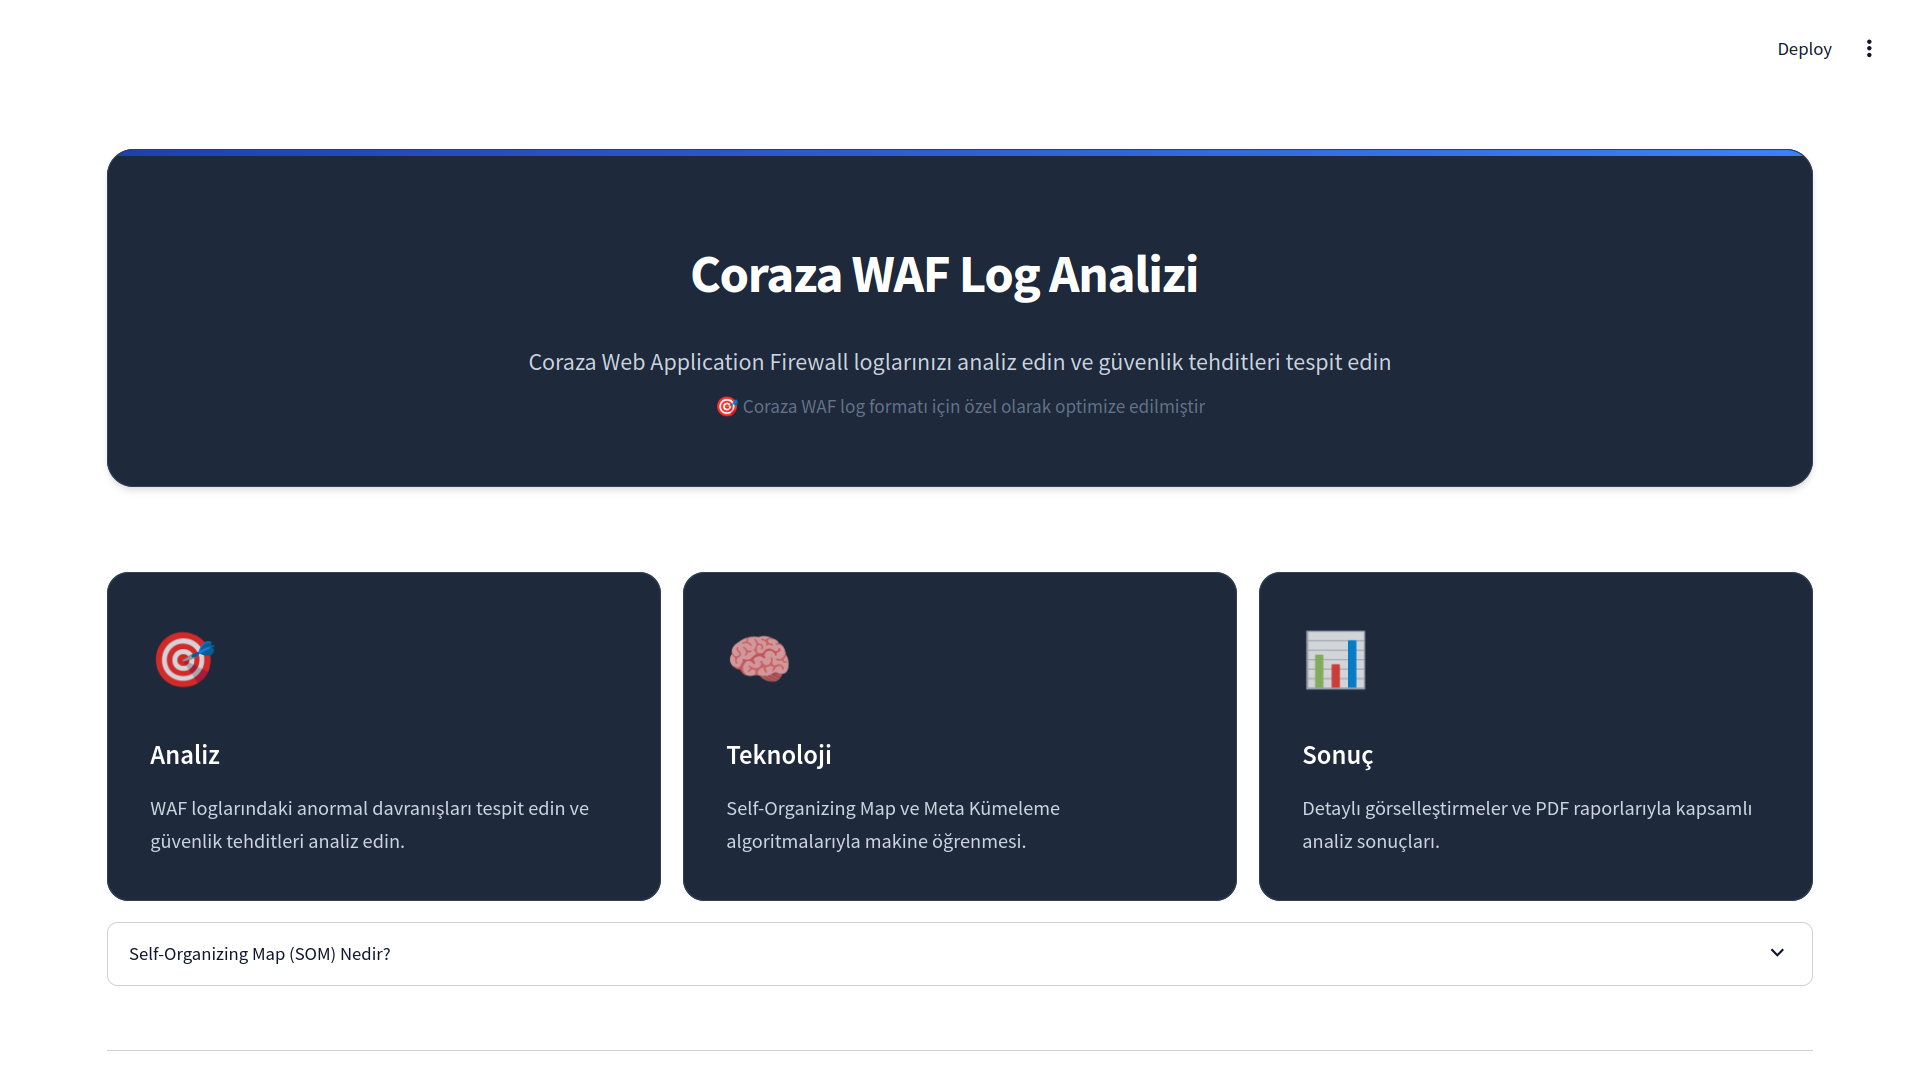
\includegraphics[width=0.8\textwidth]{images/streamlit-main-dashboard.png}
    \caption{Streamlit Ana Gösterge Paneli Görünümü}
    \label{fig:streamlit_main}
\end{figure}

\newpage

\subsubsection{Ana Arayüz Bileşenleri}

Şekil \ref{fig:streamlit_main}'de gösterilen ana arayüz şu bileşenleri içermektedir:

\begin{itemize}
    \item \textbf{Dosya Yükleme Modülü:} JSON log dosyalarının yüklenmesi
    \item \textbf{Veri İşleme Arayüzü:} Eksik veri işleme seçenekleri
    \item \textbf{SOM Parametre Ayarları:} Algoritma parametrelerinin ayarlanması
    \item \textbf{Görselleştirme Dashboard'u:} Analiz sonuçlarının sunumu
    \item \textbf{Rapor İndirme:} PDF formatında detaylı rapor
\end{itemize}


\subsubsection{İnteraktif Görselleştirmeler}

Sistem, Plotly kütüphanesi kullanılarak aşağıdaki görselleştirmeleri sağlar:

\begin{enumerate}
    \item \textbf{SOM Haritası:} U-Matrix ve component plane görselleştirmeleri
    \item \textbf{Kümeleme Sonuçları:} Meta-kümeleme algoritmaları çıktıları
    \item \textbf{Anomali Tespiti:} Quantization error dağılımları
    \item \textbf{Zaman Serisi Analizi:} Log verilerinin zamansal analizi
    \item \textbf{Boyut İndirgeme:} PCA, t-SNE ve UMAP görselleştirmeleri
\end{enumerate}

\begin{figure}[!ht]
    \centering
    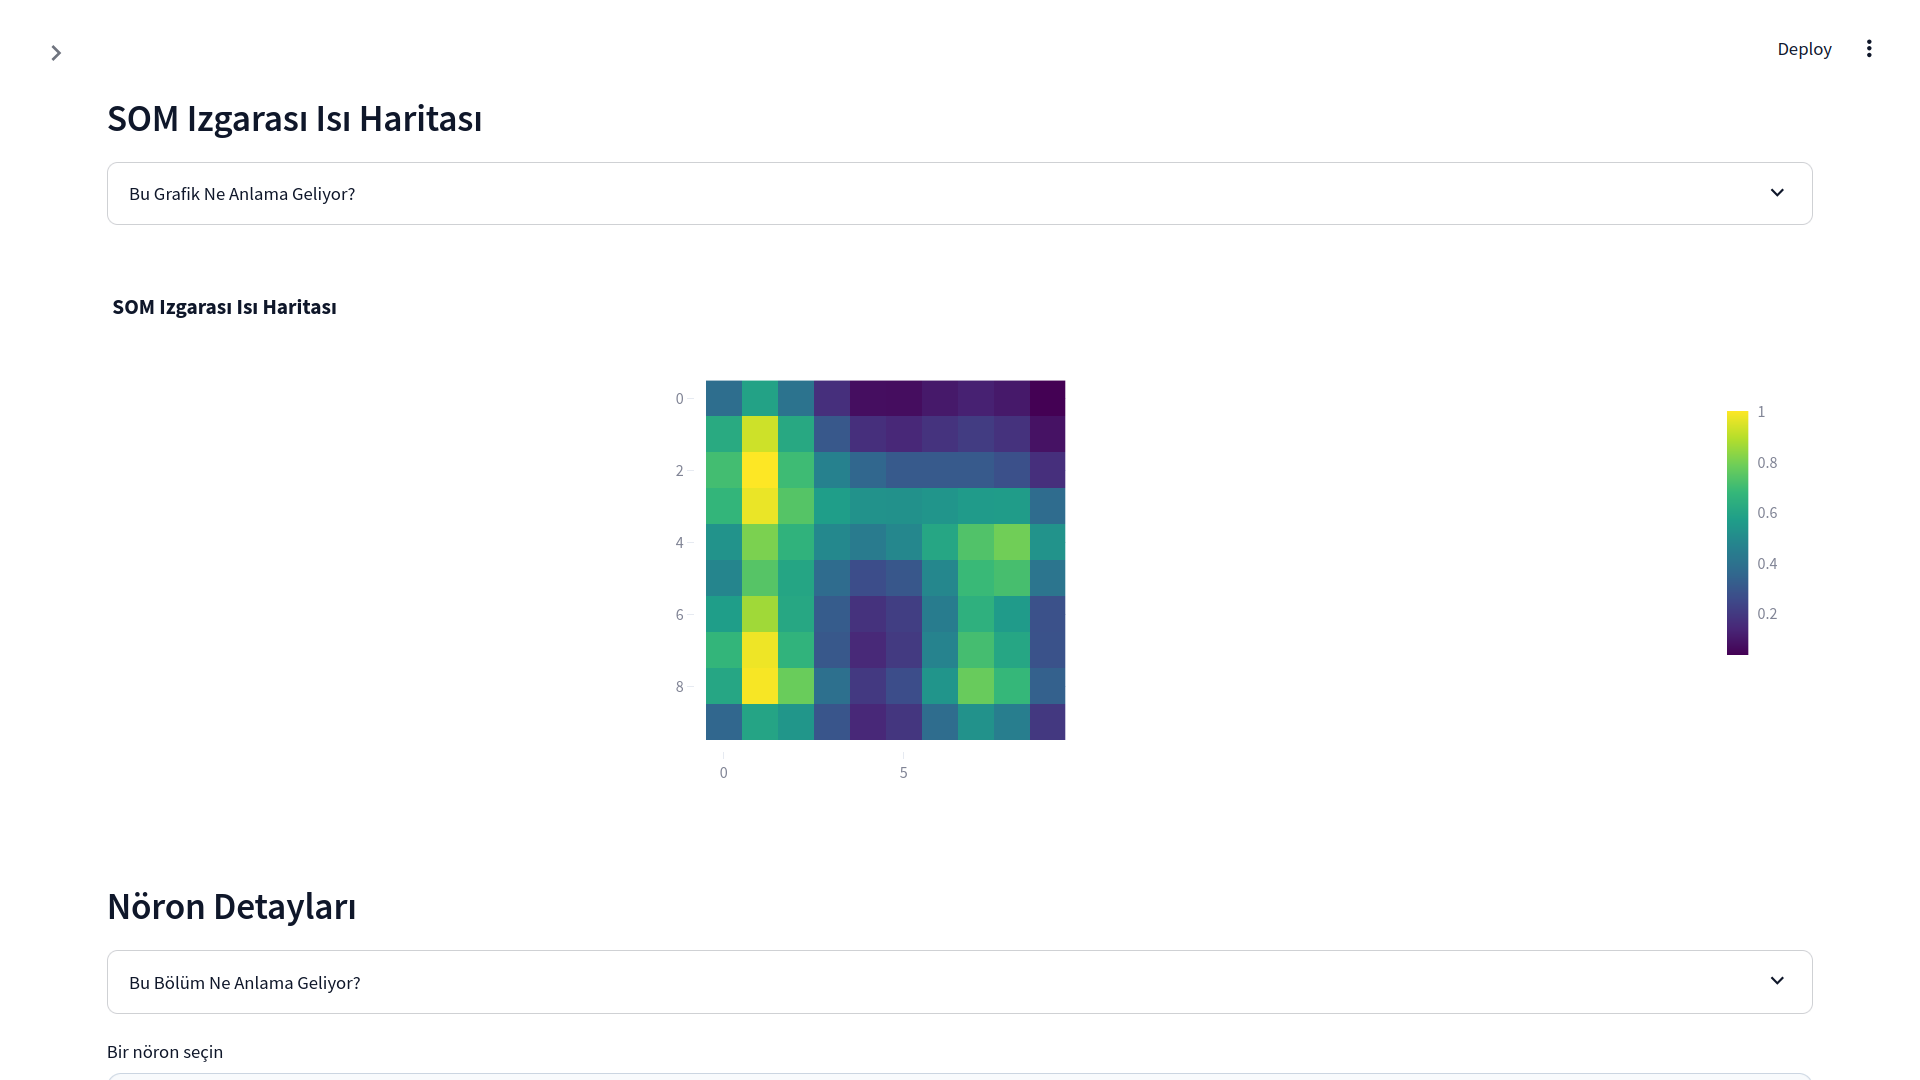
\includegraphics[width=0.9\textwidth]{images/som-visualization.png}
    \caption{SOM U-Matrix Görselleştirmesi ve Anomali Tespit Sonuçları}
    \label{fig:som_visualization}
\end{figure}

Şekil \ref{fig:som_visualization}'de SOM algoritması tarafından üretilen U-Matrix haritası ve tespit edilen anomalilerin görselleştirmesi gösterilmektedir.

\subsection{Gelişmiş Analiz Modülleri}

\subsubsection{Meta-Kümeleme Implementasyonu}

SOM çıktısı üzerinde çeşitli kümeleme algoritmaları uygulanır:

\begin{lstlisting}[language=python]
def perform_meta_clustering(som_weights, n_clusters):
    # K-means kümeleme
    kmeans = KMeans(n_clusters=n_clusters, random_state=42)
    kmeans_labels = kmeans.fit_predict(som_weights)
    
    # Hierarchical clustering
    hierarchical = AgglomerativeClustering(n_clusters=n_clusters)
    hierarchical_labels = hierarchical.fit_predict(som_weights)
    
    # DBSCAN
    dbscan = DBSCAN(eps=0.5, min_samples=5)
    dbscan_labels = dbscan.fit_predict(som_weights)
    
    return {
        'kmeans': kmeans_labels,
        'hierarchical': hierarchical_labels,
        'dbscan': dbscan_labels
    }
\end{lstlisting}

\subsubsection{Boyut İndirgeme Modülü}

Yüksek boyutlu verilerin görselleştirilmesi için üç farklı teknik kullanılır:

\begin{lstlisting}[language=python]
def apply_dimensionality_reduction(X):
    # PCA
    pca = PCA(n_components=2)
    X_pca = pca.fit_transform(X)
    
    # t-SNE
    tsne = TSNE(n_components=2, random_state=42)
    X_tsne = tsne.fit_transform(X)
    
    # UMAP
    reducer = umap.UMAP(n_components=2, random_state=42)
    X_umap = reducer.fit_transform(X)
    
    return X_pca, X_tsne, X_umap
\end{lstlisting}

\subsection{PDF Rapor Modülü}

Sistem, analiz sonuçlarını profesyonel PDF formatında sunabilen kapsamlı bir rapor modülü içerir.

\textbf{PDF Raporların Sistemdeki Kritik Rolü:}

PDF rapor modülü, SOM analiz sisteminin en önemli çıktı bileşenlerinden biridir. Bu modülün sistem için kritik önemleri şunlardır:

\begin{itemize}
    \item \textbf{Bulguların Kalıcı Dokümantasyonu:} Streamlit arayüzündeki interaktif analizlerin sonuçlarının kalıcı kayıt altına alınması
    \item \textbf{Raporlama ve Compliance:} Güvenlik analizi sonuçlarının formal raporlama gereksinimleri için standart format
    \item \textbf{Offline Erişim:} Network bağlantısı olmayan ortamlarda analiz sonuçlarının incelenebilmesi
    \item \textbf{Arşivleme ve Denetim:} Zaman içerisinde yapılan analizlerin karşılaştırmalı değerlendirmesi
    \item \textbf{Executive Summary:} Teknik olmayan karar vericiler için özet sunumları
    \item \textbf{Multi-language Support:} Türkçe karakter desteği ile yerel raporlama ihtiyaçları
\end{itemize}

\textbf{Sistem Çıktısındaki İş Akışı:}
1. Streamlit Dashboard → Analiz Sonuçları → PDF Generator → Kalıcı Rapor
2. SOM/Meta-clustering Results → Statistical Metrics → Visual Charts → Professional PDF
3. Real-time Analysis → Batch Processing → Report Template → Downloadable Document

\newpage

\subsubsection{FPDF Tabanlı Rapor Üretimi}

PDF rapor modülü, FPDF kütüphanesi kullanılarak geliştirilmiştir:

\begin{lstlisting}[language=python]
class CorazaLogPDFReport:
    def __init__(self):
        self.pdf = FPDF()
        self.pdf.add_page()
        
        # Türkçe font desteği
        font_path = self.get_turkish_font()
        if font_path:
            self.pdf.add_font('Turkish', '', font_path, uni=True)
            self.font_family = 'Turkish'
        else:
            self.font_family = 'Arial'
\end{lstlisting}

\textbf{FPDF Seçilme Nedenleri:}
\begin{itemize}
    \item Pure Python implementasyonu - external dependency minimize
    \item Unicode ve Türkçe karakter desteği
    \item Matplotlib figure entegrasyonu
    \item Memory-efficient processing
    \item Cross-platform compatibility
\end{itemize}

\subsubsection{Rapor İçeriği}

Otomatik oluşturulan PDF rapor aşağıdaki bölümleri içerir:

\begin{enumerate}
    \item \textbf{Kapak Sayfası:} Proje bilgileri ve oluşturma tarihi
    \item \textbf{Veri Özeti:} İşlenen veri miktarı ve özellik istatistikleri
    \item \textbf{SOM Analizi:} Eğitim parametreleri ve performans metrikleri
    \item \textbf{Meta-Kümeleme Sonuçları:} Algoritma karşılaştırmaları
    \item \textbf{Gelişmiş Analizler:} Stabilite ve doğrulama sonuçları
    \item \textbf{Görselleştirmeler:} Matplotlib figürlerinin entegrasyonu
    \item \textbf{Sonuç ve Öneriler:} Analiz çıkarımları
\end{enumerate}

\newpage

\subsubsection{Görsel Entegrasyonu}

Matplotlib figürleri Base64 encoding ile PDF'e gömülür:

\begin{lstlisting}[language=python]
def add_matplotlib_figure(self, fig, title, width=150):
    # Figürü BytesIO tamponuna kaydet
    img_buffer = io.BytesIO()
    fig.savefig(img_buffer, format='png', dpi=300,
               bbox_inches='tight', facecolor='white')
    img_buffer.seek(0)

    # Geçici dosyaya kaydet
    with tempfile.NamedTemporaryFile(delete=False, suffix='.png') as tmp_file:
        tmp_file.write(img_buffer.getvalue())
        tmp_file_path = tmp_file.name
    
    self.pdf.image(tmp_file_path, x=30, w=width)
    self.pdf.ln(5)
    
    # Geçici dosyayı sil
    os.unlink(tmp_file_path)
\end{lstlisting}

\subsubsection{Çoklu Dil Desteği}

Sistem, Türkçe karakter desteği için özel font yönetimi içerir:

\begin{lstlisting}[language=python]
def get_turkish_font(self):
    font_paths = [
        '/usr/share/fonts/truetype/dejavu/DejaVuSans.ttf',
        './fonts/DejaVuSans.ttf',
        './static_fonts/DejaVuSans.ttf'
    ]
    
    for path in font_paths:
        if os.path.exists(path):
            return path
    return None
\end{lstlisting}
